\documentclass{article}
\usepackage{graphicx}
\usepackage{amsmath}
\usepackage[parfill]{parskip}
\usepackage{hyperref}
\usepackage[useregional]{datetime2}

\usepackage[T1]{fontenc}
\usepackage{tgbonum}

\usepackage{listings}
\usepackage{xcolor}

% Define a custom color
\definecolor{backcolour}{rgb}{0.95,0.95,0.92}
\definecolor{codegreen}{rgb}{0,0.6,0}

% Define a custom style
\lstdefinestyle{myStyle}{
    backgroundcolor=\color{backcolour},   
    commentstyle=\color{codegreen},
    basicstyle=\ttfamily\footnotesize,
    breakatwhitespace=false,         
    breaklines=true,                 
    keepspaces=true,                 
    numbers=left,       
    numbersep=5pt,                  
    showspaces=false,                
    showstringspaces=false,
    showtabs=false,                  
    tabsize=2,
}

% Use \lstset to make myStyle the global default
\lstset{style=myStyle}

\usepackage{biblatex}
\addbibresource{references.bib}

\graphicspath{ {./figures/} }

\title{COMP.SEC.110 Cyber Security II
    \large Practical Exercise: Public Key Infrastructure\!
}
\author{Cuong Nguyen\\ \href{mailto:cuong.nguyen@tuni.fi}{cuong.nguyen@tuni.fi} 
        \and Mahibul Momin\\ \href{mailto:mahibul.momin@tuni.fi}{mahibul.momin@tuni.fi}
}

\begin{document}
    
\maketitle
\tableofcontents
\newpage

\listoffigures
\newpage

% Content of report would be written here
% \section{Lab Tasks: Attacks}
\subsection{Task 1 --- Observing HTTP Request}
%
\begin{figure}
    \centering
    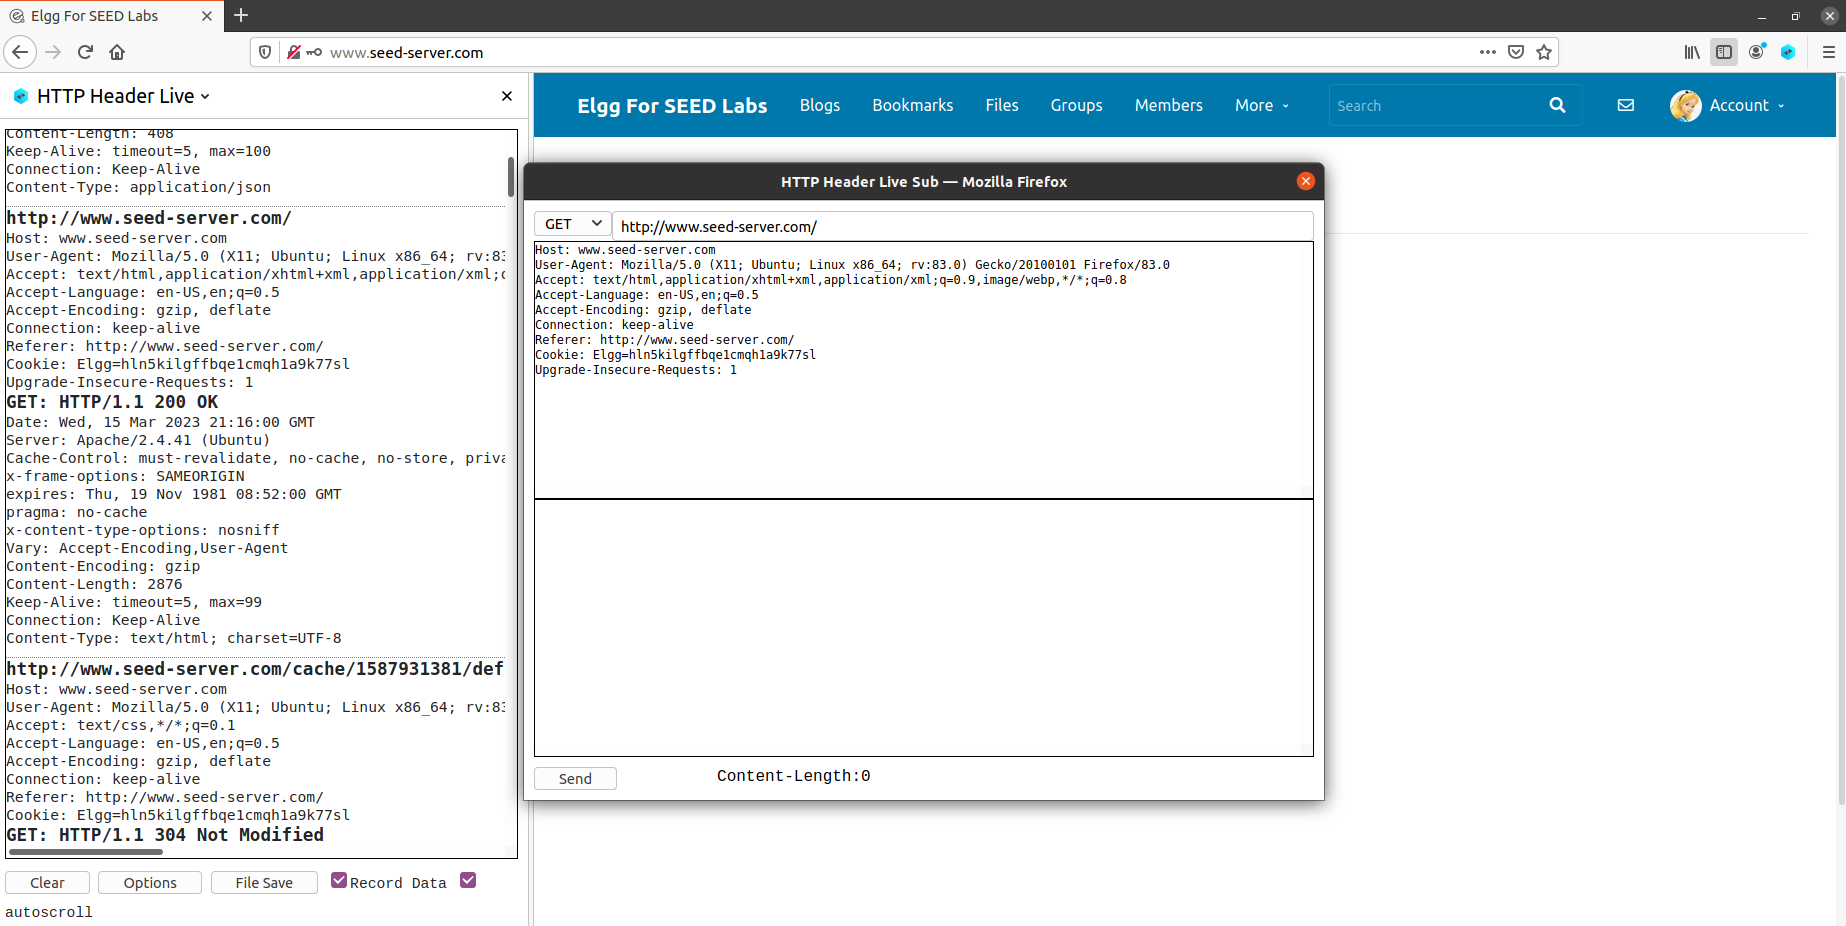
\includegraphics[width=\textwidth,height=\textheight,keepaspectratio]
    {figures/HTTP_GET.png}
    \caption{HTTP GET request in Elgg.}\label{fig:http_get}
\end{figure}

\begin{figure}
    \centering
    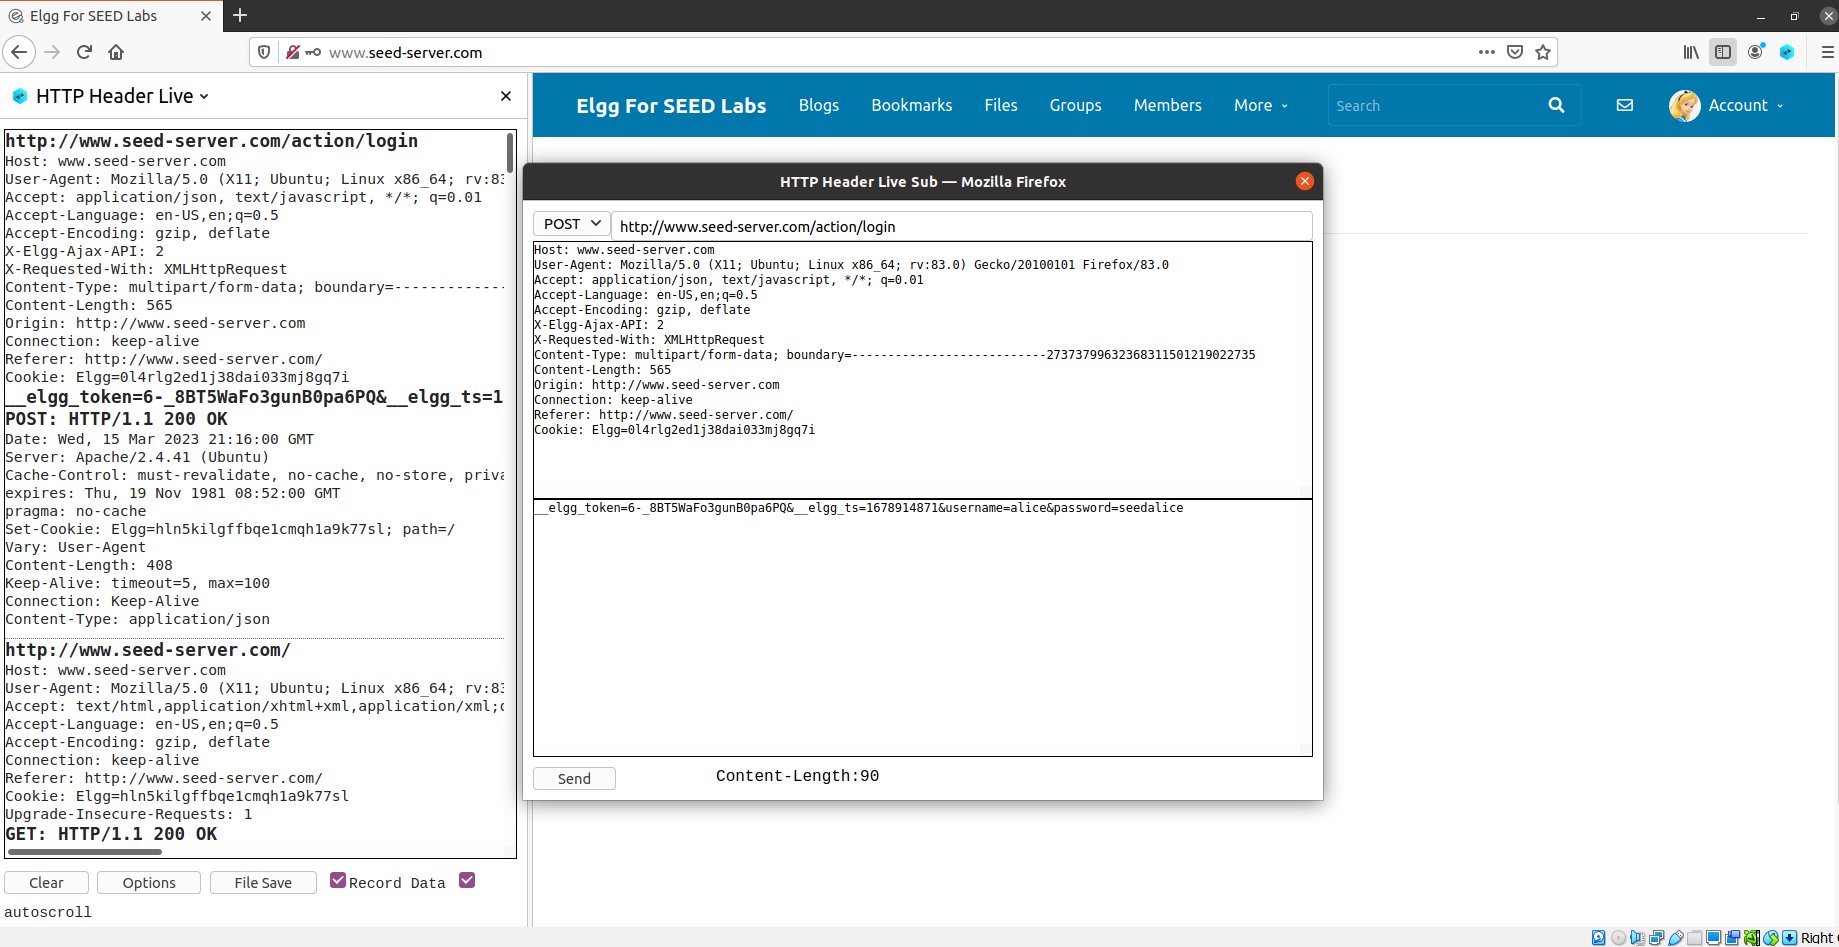
\includegraphics[width=\textwidth,height=\textheight,keepaspectratio]
    {figures/HTTP_POST.png}
    \caption{HTTP POST request in Elgg.}\label{fig:http_post}
\end{figure}

In the HTTP POST request, in this case we was trying to log in with a valid
authentication (username: \emph{alice}, password: \emph{seedalice}), it requires
a pair of parameters:{\fontfamily{qcr}\selectfont username} and
{\fontfamily{qcr}\selectfont password} (see \autoref{fig:http_post}).
On the other hand, a HTTP GET request does not require any parameters
(see \autoref{fig:http_get}).
% ...
% \section{Task 2 --- Generating a Certificate Request for Your Web Server}
%
\begin{lstlisting}[language=bash,caption=A command generating CSR for the server]
openssl req -newkey rsa:2048 -sha256 \
    -keyout server.key -out server.csr \
    -subj "/CN=www.student22.com/O=Student22 Inc./C=US" \
    -passout pass:dees \
    -addext "subjectAltName = DNS:www.student22.com,\
                            DNS:www.student22cuong.com,\
                            DNS:www.student22mahibul.com"
\end{lstlisting}

\begin{figure}
    \centering
    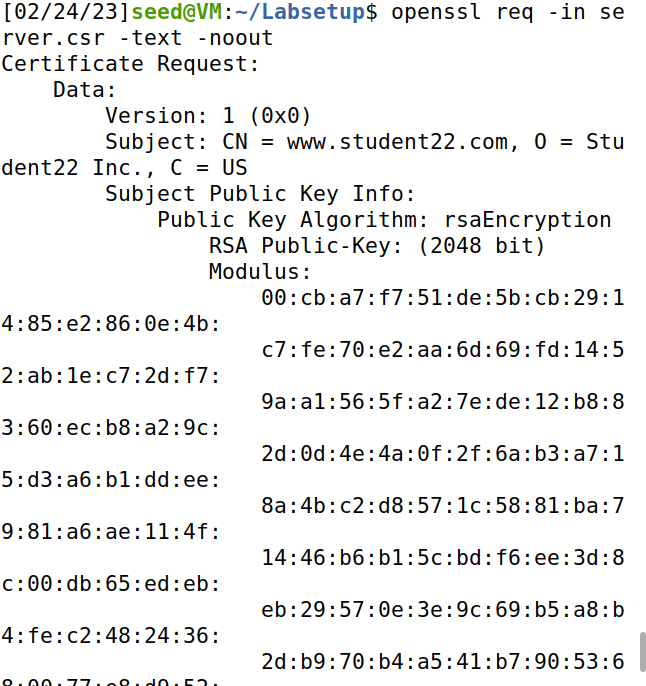
\includegraphics[height=\textheight,width=\textwidth,keepaspectratio]
    {figures/server_csr.png}
    \caption{Certificate Signing Request for the server
    {\fontfamily{qcr}\selectfont www.student22.com}.}
    \label{fig:server_csr}
\end{figure}

Two alternative names, {\fontfamily{qcr}\selectfont www.student22cuong.com} and
{\fontfamily{qcr}\selectfont www.student22mahibul.com}, are included
in the {\fontfamily{qcr}\selectfont openssl ca} command.
\autoref{fig:server_csr} shows partly the Certificate Signing Request
(CSR) for the server {\fontfamily{qcr}\selectfont www.student22.com}.

\section{Lab Tasks: Attacks}
\subsection{Task 1 --- Observing HTTP Request}
%
\begin{figure}
    \centering
    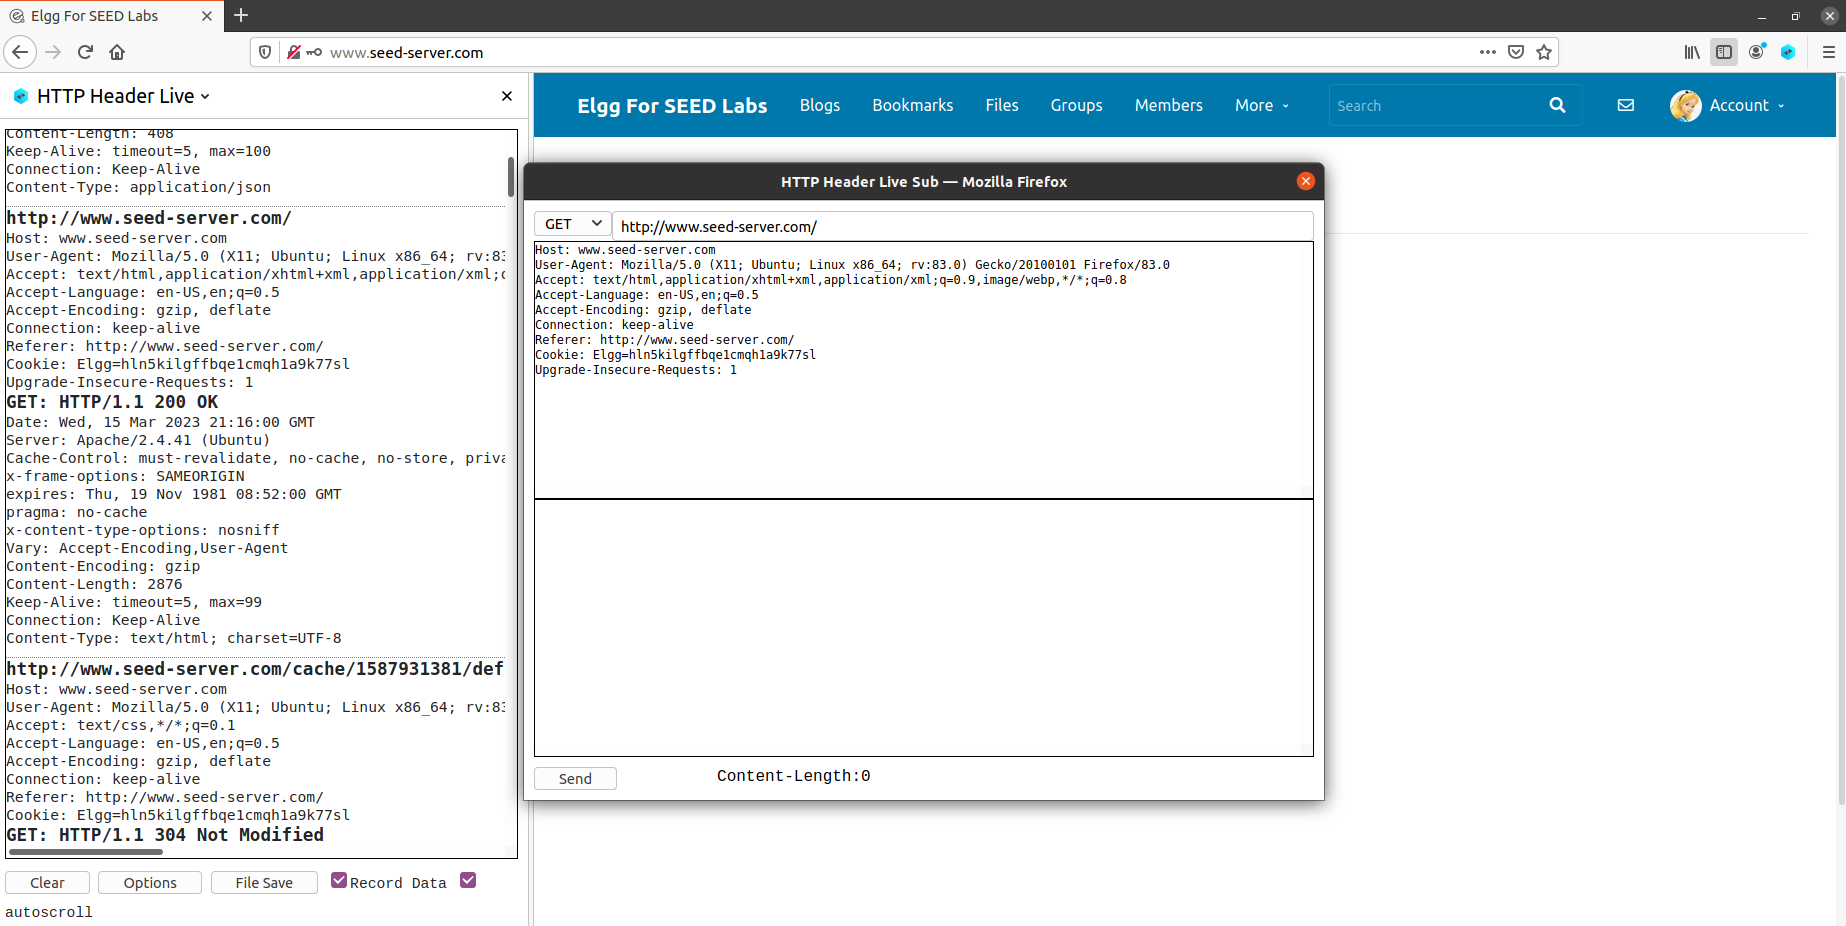
\includegraphics[width=\textwidth,height=\textheight,keepaspectratio]
    {figures/HTTP_GET.png}
    \caption{HTTP GET request in Elgg.}\label{fig:http_get}
\end{figure}

\begin{figure}
    \centering
    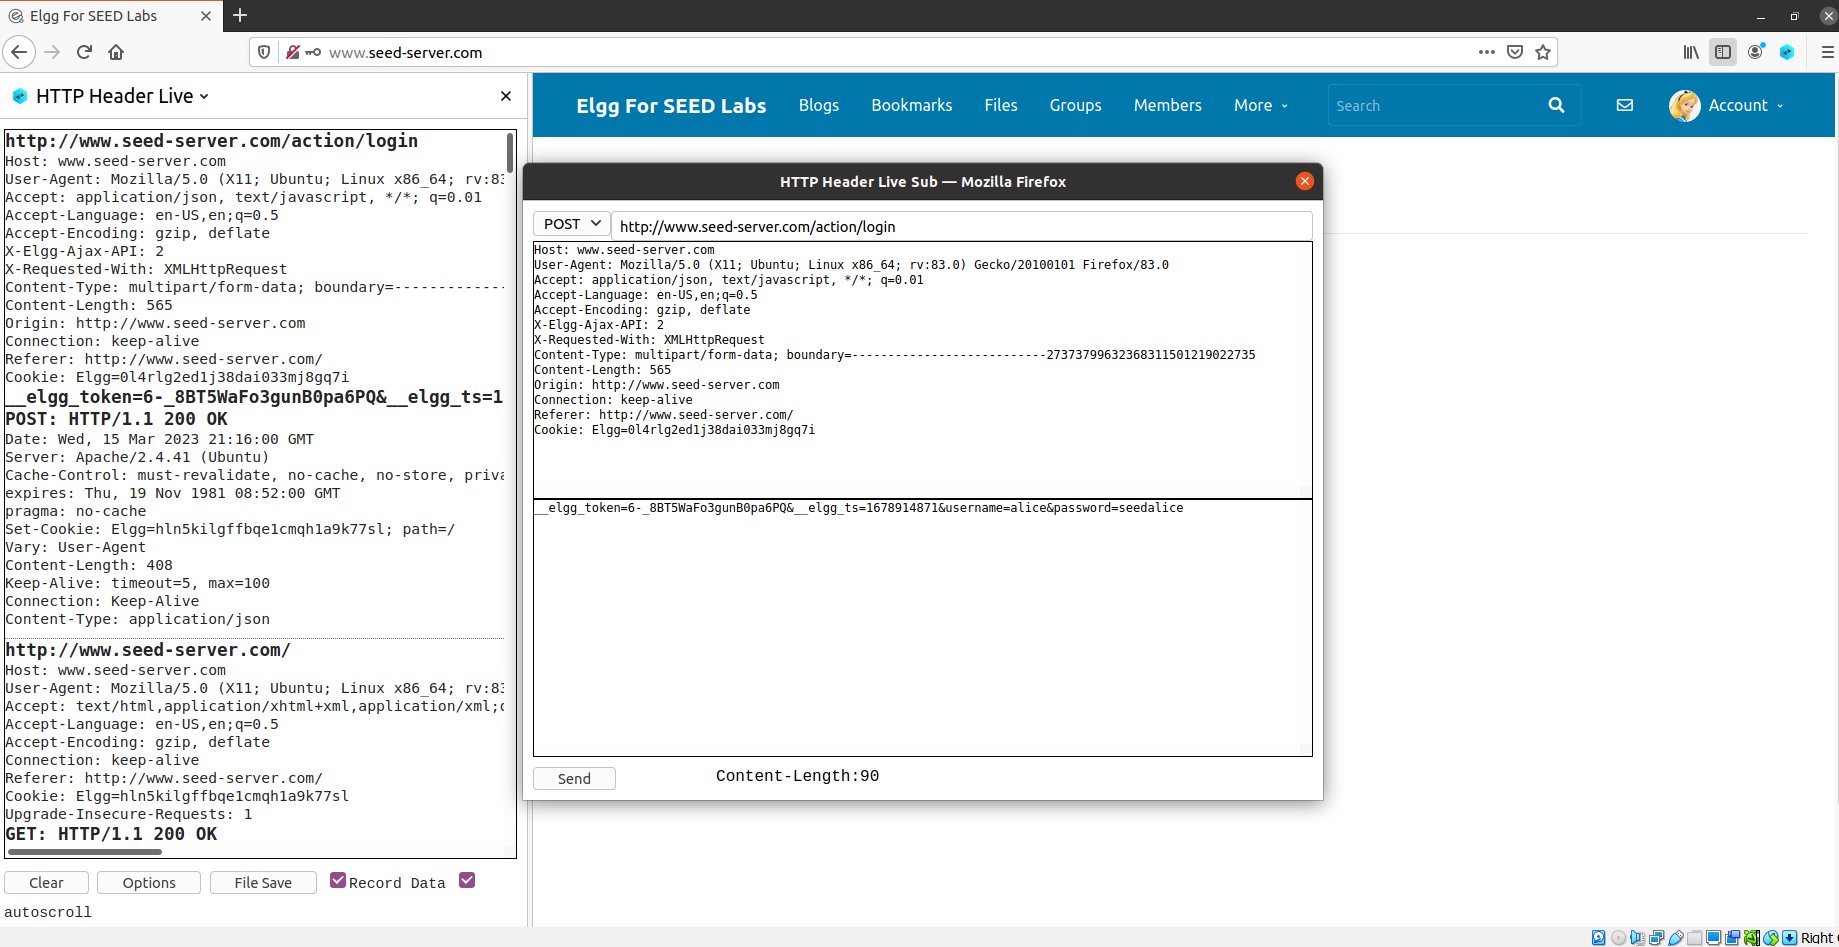
\includegraphics[width=\textwidth,height=\textheight,keepaspectratio]
    {figures/HTTP_POST.png}
    \caption{HTTP POST request in Elgg.}\label{fig:http_post}
\end{figure}

In the HTTP POST request, in this case we was trying to log in with a valid
authentication (username: \emph{alice}, password: \emph{seedalice}), it requires
a pair of parameters:{\fontfamily{qcr}\selectfont username} and
{\fontfamily{qcr}\selectfont password} (see \autoref{fig:http_post}).
On the other hand, a HTTP GET request does not require any parameters
(see \autoref{fig:http_get}).
\section{Task 2 --- Generating a Certificate Request for Your Web Server}
%
\begin{lstlisting}[language=bash,caption=A command generating CSR for the server]
openssl req -newkey rsa:2048 -sha256 \
    -keyout server.key -out server.csr \
    -subj "/CN=www.student22.com/O=Student22 Inc./C=US" \
    -passout pass:dees \
    -addext "subjectAltName = DNS:www.student22.com,\
                            DNS:www.student22cuong.com,\
                            DNS:www.student22mahibul.com"
\end{lstlisting}

\begin{figure}
    \centering
    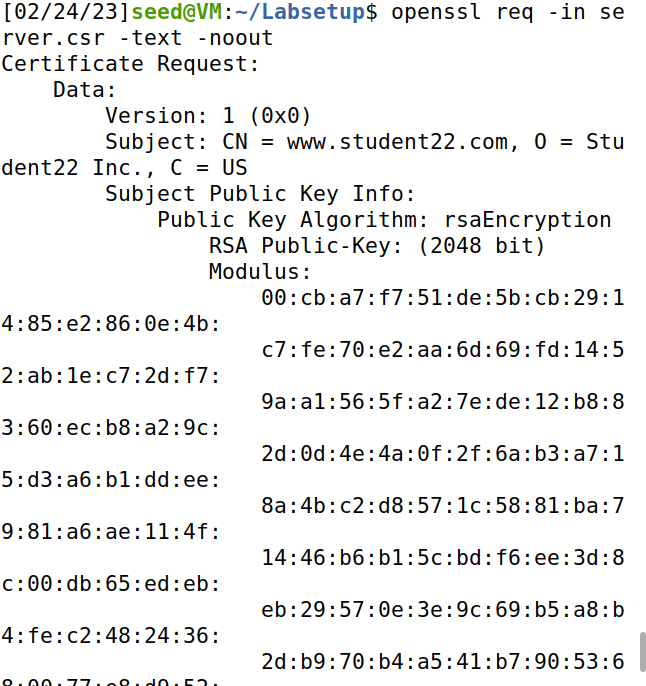
\includegraphics[height=\textheight,width=\textwidth,keepaspectratio]
    {figures/server_csr.png}
    \caption{Certificate Signing Request for the server
    {\fontfamily{qcr}\selectfont www.student22.com}.}
    \label{fig:server_csr}
\end{figure}

Two alternative names, {\fontfamily{qcr}\selectfont www.student22cuong.com} and
{\fontfamily{qcr}\selectfont www.student22mahibul.com}, are included
in the {\fontfamily{qcr}\selectfont openssl ca} command.
\autoref{fig:server_csr} shows partly the Certificate Signing Request
(CSR) for the server {\fontfamily{qcr}\selectfont www.student22.com}.
\section{Task3 --- Encryption Mode --- ECB vs. CBC}
%

\begin{figure}
    \centering
    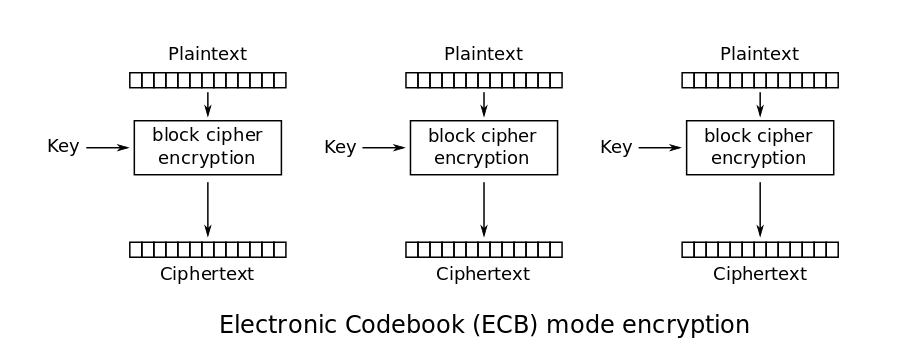
\includegraphics[height=\textheight,width=\textwidth,keepaspectratio]
    {figures/ECB_encryption.png}
    \caption{Electronic Codebook (ECB) mode encryption~\cite{cipher_mode_wiki}.}
    \label{fig:ecb_mode}
\end{figure}

\begin{figure}
    \centering
    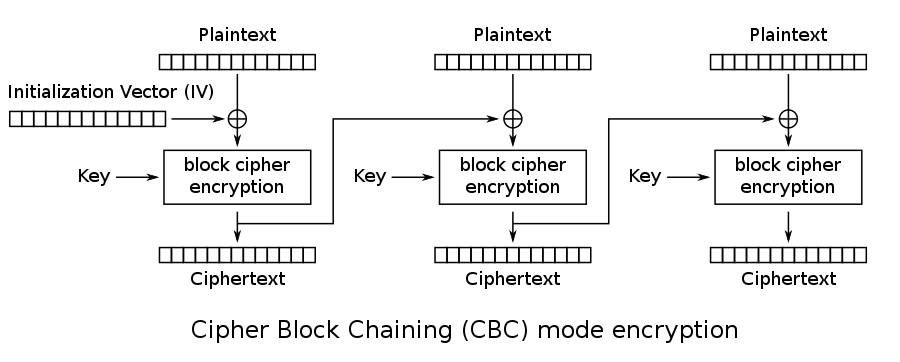
\includegraphics[height=\textheight,width=\textwidth,keepaspectratio]
    {figures/CBC_encryption.png}
    \caption{Cipher Block Chaining (CBC) mode encryption~\cite{cipher_mode_wiki}.}
    \label{fig:cbc_mode}
\end{figure}

In the electronic codebook (ECB) mode, the plaintext is splitted into
blocks which are encrypted separately, as shown in \autoref{fig:ecb_mode}.
The drawback of this mode is a lack of diffusion~\cite{cipher_mode_wiki}.
Identical plaintext blocks are encrypted into identical ciphertext blocks,
exposing the data pattern easily~\cite{ecb_cbc_example}. Two examples below
illustrate this disadvantage. In more detail, while encrypting a bitmap
image, ECB mode encrypts identically-colored original pixels to a uniform
pattern. Hence, the overall pattern of the image can be detected~\cite{cipher_mode_wiki}.
Note that only the pattern of a image which contains large uniform areas
can be discerned easily. Since if a image contains pixels with variant 
color, its encrypted version will look noisy with pseudo-randomly colored
pixels.

In the cipher block chaining (CBC) mode, each plaintext block is XORed with
the previous ciphertext block before being encrypted~\cite{cipher_mode_wiki},
as shown in \autoref{fig:cbc_mode}.
In addition, the first plaintext block is XORed with the initial vector (IV)
before being encrypted. Thus, each block of ciphertext depends on all
previous ciphertext blocks~\cite{cipher_mode_wiki}. This relationship prevents
identical plaintext blocks from producing identical ciphertext blocks~\cite{ecb_cbc_example}.

In the next two subsections, we will observe examples in which bitmap images are
encrypted with both cipher modes.

\subsection{Using picture {\fontfamily{qcr}\selectfont pic\_original.bmp}}
%
\begin{lstlisting}[language=Bash, caption=Commands generating
    {\fontfamily{qcr}\selectfont pic\_cbc.bmp}, label={lst:pic_cbc}]
$ openssl enc -e -des-cbc -salt -pbkdf2 -kfile password.txt \
    -in pic_original.bmp -out pic_original.bmp.cbc # encrypt the original picture
$ head -c 54 pic_original.bmp > header # create a file containing header of a bitmap image
$ tail -c +55 pic_original.bmp.cbc > cbc_body # create a file containing body of an encrypted image

# combine the original header and the encrypted body to
# create a complete encrypted bitmap image
$ cat header cbc_body > pic_cbc.bmp
\end{lstlisting}

Given an original image (\autoref{fig:original_pic}), we can obtain its
overall pattern though it was encrypted with ECB mode, shown in \autoref{fig:ecb_pic}.
Since the original image contains three large uniform-color areas
, including an ellipse (red), a rectangular (green), and a background (white)
, the patterns of these
3 areas are splitted clearly. The reason behind is that uniform areas of
red (green, or white) pixels are encrypted into colored uniform areas, so
we still see these shapes but with another color.

On the other hand, by looking at the output of CBC mode (\autoref{fig:cbc_pic}), we cannot
detect the pattern of the original image as the encrypted version now looks
very noisy.

\begin{lstlisting}[language=Bash, caption=Commands generating
    {\fontfamily{qcr}\selectfont pic\_ecb.bmp}, label={lst:pic_ecb}]
$ openssl enc -e -des-ecb -salt -pbkdf2 -kfile password.txt \
    -in pic_original.bmp -out pic_original.bmp.ecb # encrypt the original picture
$ head -c 54 pic_original.bmp > header
$ tail -c +55 pic_original.bmp.ecb > ecb_body
$ cat header ecb_body > pic_ecb.bmp
\end{lstlisting}

\begin{figure}
    \centering
    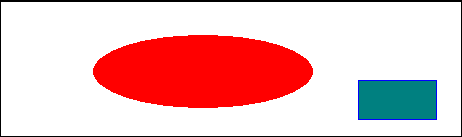
\includegraphics[height=\textheight,width=\textwidth,keepaspectratio]
    {figures/pic_original.png}
    \caption{The original picture.}\label{fig:original_pic}
\end{figure}

\begin{figure}
    \centering
    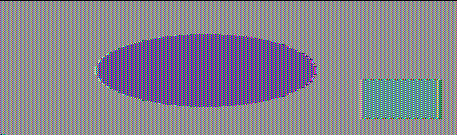
\includegraphics[height=\textheight,width=\textwidth,keepaspectratio]
    {figures/pic_ecb.png}
    \caption{The ECB-mode encrypted picture.}\label{fig:ecb_pic}
\end{figure}

\begin{figure}
    \centering
    
\includegraphics[height=\textheight,width=\textwidth,keepaspectratio]
    {figures/pic_cbc.png}
    \caption{The CBC-mode encrypted picture.}\label{fig:cbc_pic}
\end{figure}

\subsection{Using picture {\fontfamily{qcr}\selectfont snail.bmp}}
%
\begin{lstlisting}[language=Bash, caption=Commands generating
    {\fontfamily{qcr}\selectfont snail\_cbc.bmp}, label={
        lst:snail_cbc
    }]
$ openssl enc -e -des-cbc -salt -pbkdf2 -kfile password.txt \
    -in snail.bmp -out snail.bmp.cbc # encrypt the original picture
$ head -c 54 snail.bmp > snail_header
$ tail -c +55 snail.bmp.cbc > snail_cbc_body
$ cat snail_header snail_cbc_body > snail_cbc.bmp
\end{lstlisting}

Given an original image (\autoref{fig:snail}), we can obtain its
overall pattern though it was encrypted with ECB mode, shown in
\autoref{fig:snail_ecb}.
Since the original image contains two large uniform-color areas
, including the snail (yellow) and the background (white), the patterns of these
2 areas are splitted clearly. The reason behind is that uniform areas of
yellow (or white) pixels are encrypted into colored uniform areas, so
we still see these shapes but with another color. In this case, the snail
itself produced a noisy encrypted pattern as color of the snail is variant.

On the other hand, by looking at the output of CBC mode
(\autoref{fig:snail_cbc}),
we cannot detect the pattern of the original image as the encrypted
version now looks very noisy.

\begin{lstlisting}[language=Bash, caption=Commands generating
    {\fontfamily{qcr}\selectfont snail\_ecb.bmp}, label={
        lst:snail_ecb
    }]
$ openssl enc -e -des-ecb -salt -pbkdf2 -kfile password.txt \
    -in snail.bmp -out snail.bmp.ecb # encrypt the original picture
$ head -c 54 snail.bmp > snail_header
$ tail -c +55 snail.bmp.ecb > snail_ecb_body
$ cat snail_header snail_ecb_body > snail_ecb.bmp
\end{lstlisting}

\begin{figure}
    \centering
    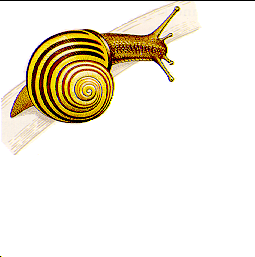
\includegraphics[height=\textheight,width=\textwidth,keepaspectratio]
    {figures/snail.png}
    \caption{The Bitmap picture of a snail.}\label{fig:snail}
\end{figure}

\begin{figure}
    \centering
    
\includegraphics[height=\textheight,width=\textwidth,keepaspectratio]
    {figures/snail_cbc.png}
    \caption{The CBC-mode encrypted picture of a snail.}\label{fig:snail_cbc}
\end{figure}

\begin{figure}
    \centering
    
\includegraphics[height=\textheight,width=\textwidth,keepaspectratio]
    {figures/snail_ecb.png}
    \caption{The ECB-mode encrypted picture of a snail.}\label{fig:snail_ecb}
\end{figure}
\section{Lab Tasks: Defense}
%
\subsection{Task 4: Enabling Elgg's Countermeasure}
%
\begin{figure}
    \centering
    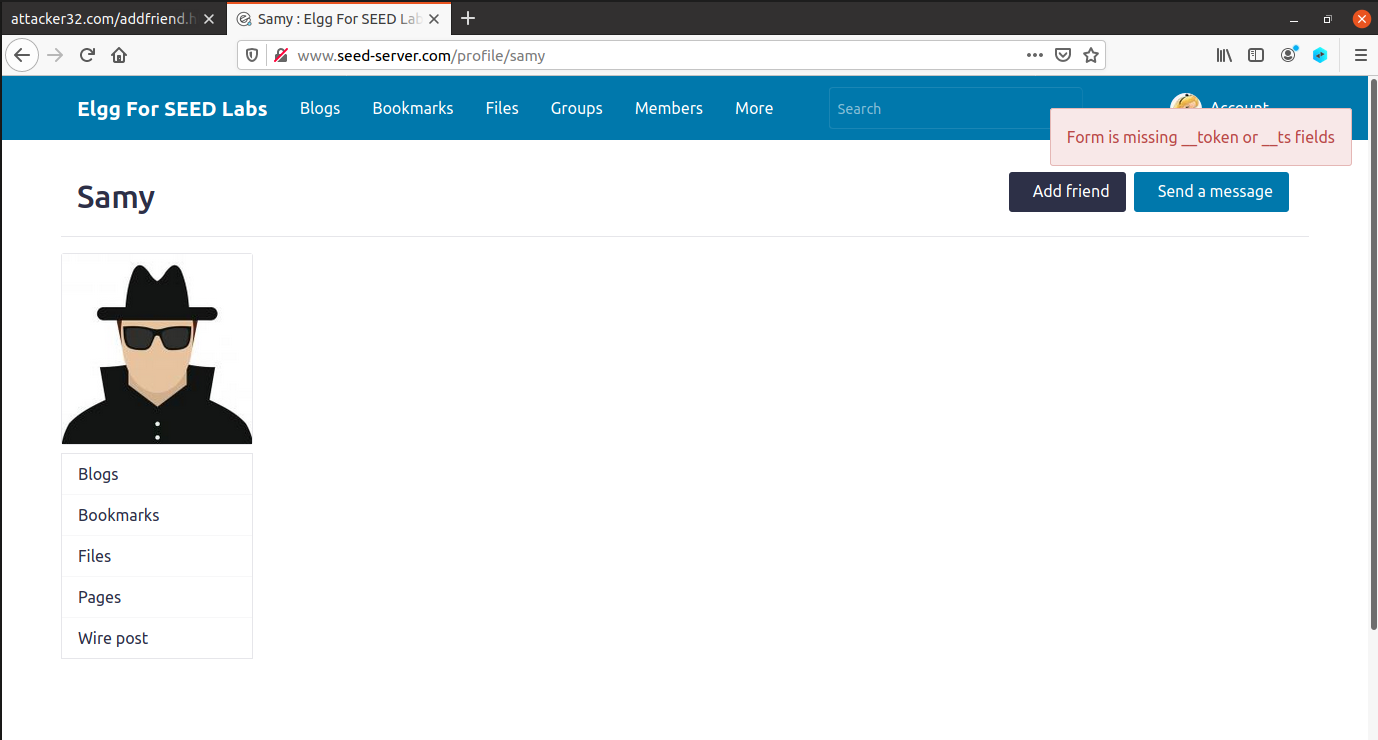
\includegraphics[height=\textheight,width=\textwidth,keepaspectratio]
    {figures/add_friend_countermeasure.png}
    \caption{CSFR countermeasure prevents the HTTP GET request forging attack.}
    \label{fig:counter_add_friend}
\end{figure}

\begin{figure}
    \centering
    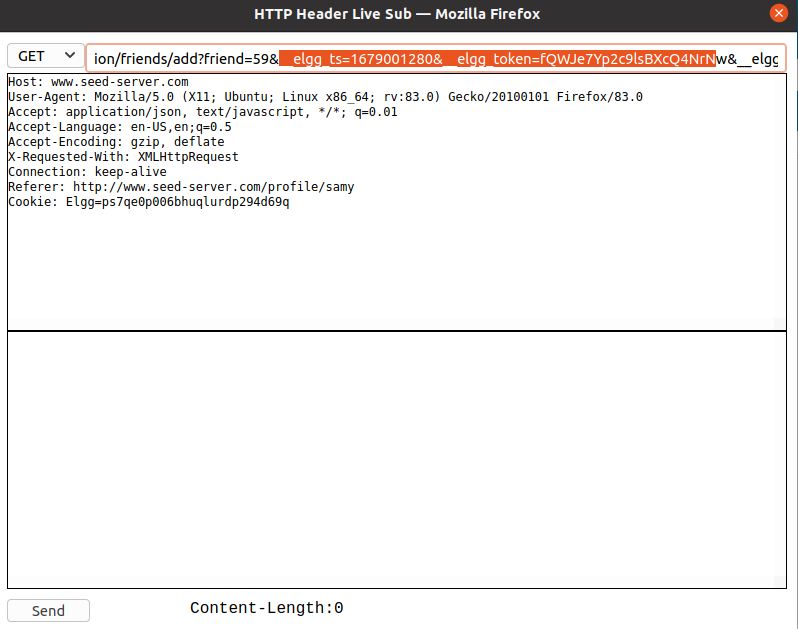
\includegraphics[height=\textheight,width=\textwidth,keepaspectratio]
    {figures/token_http_get.png}
    \caption{Secret tokens embedded in URL of an HTTP GET request.}
    \label{fig:secret_token}
\end{figure}

\begin{figure}
    \centering
    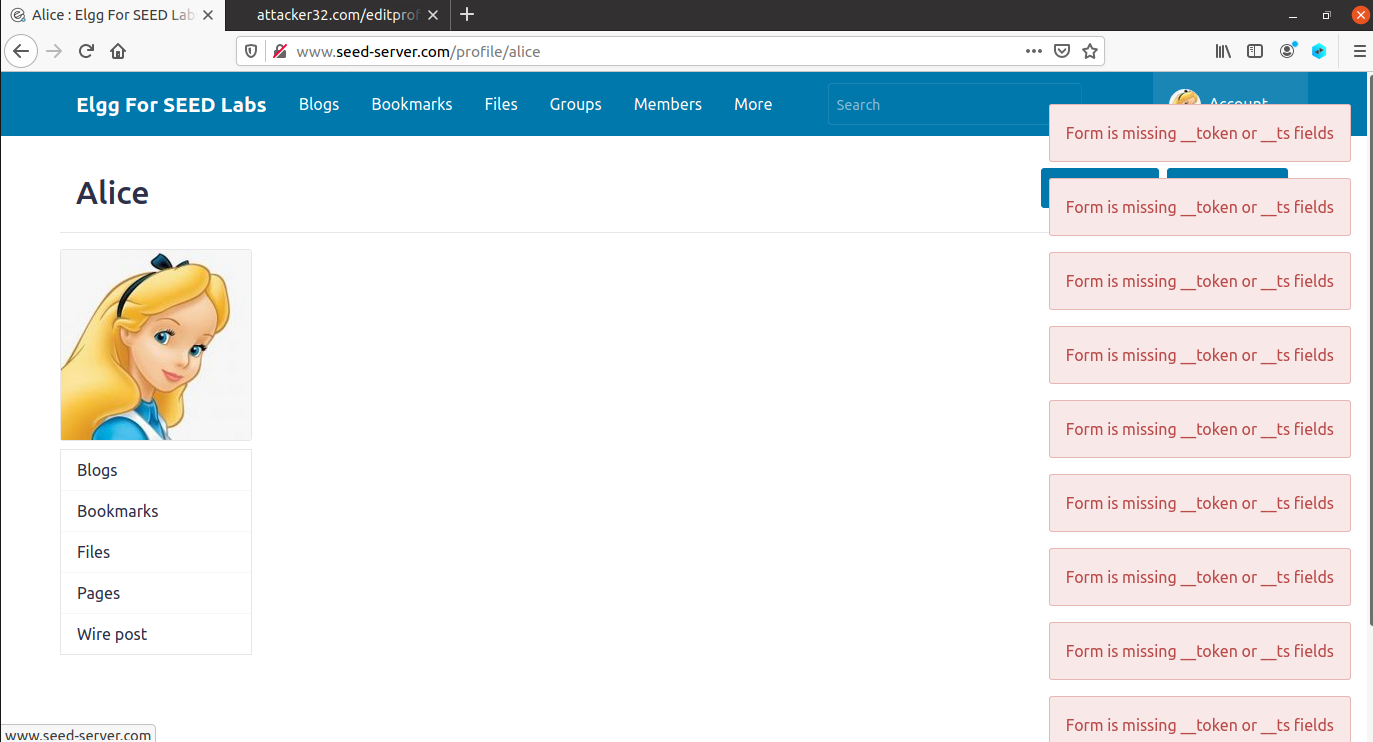
\includegraphics[height=\textheight,width=\textwidth,keepaspectratio]
    {figures/edit_profile_countermeasure.png}
    \caption{CSFR countermeasure prevents the HTTP POST request forging attack.}
    \label{fig:counter_edit_profile}
\end{figure}

After turn on the CSRF countermeasure by commenting out the {\fontfamily{qcr}\selectfont
return} line, it turned out that we cannot do CSFR attacks like above. For instance,
when we conducted the {\fontfamily{qcr}\selectfont add\_friend} attack, Elgg page raised
an alert noticing that {\fontfamily{qcr}\selectfont \_\_elgg\_token} and
{\fontfamily{qcr}\selectfont \_\_elgg\_ts} fields are missing
(see \autoref{fig:counter_add_friend}). In the case of {\fontfamily{qcr}\selectfont edit\_profile}
attack, as the attacker's page is reloaded, the forged POST request is re-triggered, so
a chain of red alerts was shown (see \autoref{fig:counter_edit_profile}).

Logged-in as Alice and then pressed the {\fontfamily{qcr}\selectfont Add friend} button,
we captured a HTTP GET request including two secret tokens (see \autoref{fig:secret_token}).

\begin{itemize}
    \item \_\_elgg\_ts: 1679001280
    \item \_\_elgg\_token: fQWJe7Yp2c9lsBXcQ4NrNw
\end{itemize}

The attacker cannot send these secret tokens as he does not know their values.
The access control system of browser does not allow the JavaScript code in the
malicious webpage access any content in Elgg's pages. In addition, as secret
tokens are hashed value of \emph{site secret value, timestamp, user session ID,
and random generated session string}, it is nearly impossible to guess. On the
other hand, if the attacker wants to do brute-force based on the hash collision,
he has to wait in a long time. Meanwhile, these two secret values have changed
periodcally or once the user starts a new session. So if the attacker can
brute-force these two hash values, these finding won't be valid anymore.

% 01011101 01010001 00101011 10110010
% should be replaced as 01011101 01010001 00101011 10110011
% changed the LSB
\section{Task 5 --- Error Propagation --- Corrupted Cipher Text}
\subsection{Our guess}
%
\begin{table}
    \centering
    \begin{tabular}{|l|l|}
        \hline
        Mode & Effect of bit error at ciphertext block \(C_i\)\\
        \hline
        ECB & A whole plaintext block \(i\) is affected. The corrupted bits are randomized
        within a block.\\
        \hline
        CBC & Two plaintext blocks are affected. A specific corrupted bit appears in
        the next block. Random bit errors appears at block \(i\).\\
        \hline
        CFB & Specific bit error appears at block \(i\).
            Random bit errors appear at block \(i+1\) (the next block).\\
        \hline
        OFB & Specific bit error at plaintext block \(i\).\\
        \hline
    \end{tabular}
    \caption{Our guess of the effect of bit error at ciphertext.}
    \label{tab:error_bit_guess}
\end{table}

Based on the workflow of cipher modes (see \autoref{fig:cbc_dec}, \autoref{fig:ecb_dec},
\autoref{fig:cfb_dec}, \autoref{fig:ofb_dec}), we made our prediction about how the corrupted
bit appears in the decrypted text (see \autoref{tab:error_bit_guess}).
\subsection{Observation}
%
\begin{lstlisting}[language=Bash, caption=A script generating {\fontfamily{qcr}
    \selectfont plaintext.txt}., label={lst:plaintext_generation} ]
    $ python -c "print('ccccccccccccccc '*100)" > plaintext.txt
\end{lstlisting}

\begin{figure}
    \centering
    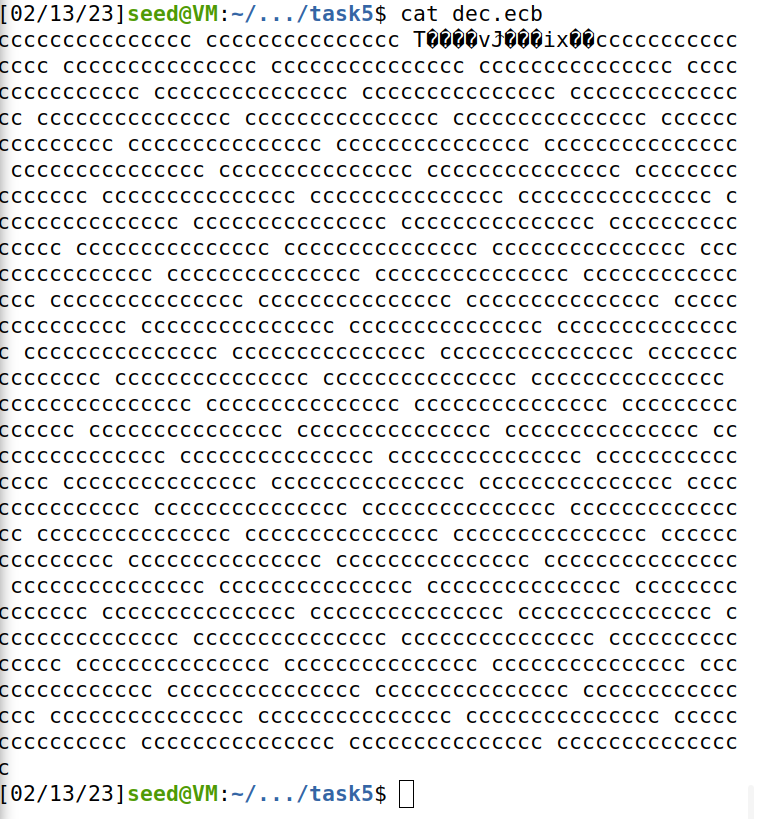
\includegraphics[height=\textheight,width=\textwidth,keepaspectratio]
    {figures/dec_ecb_task5.png}
    \caption{Decrypted text with corrupted bits using ECB mode.}\label{fig:corrupted_ecb}
\end{figure}

\begin{figure}
    \centering
    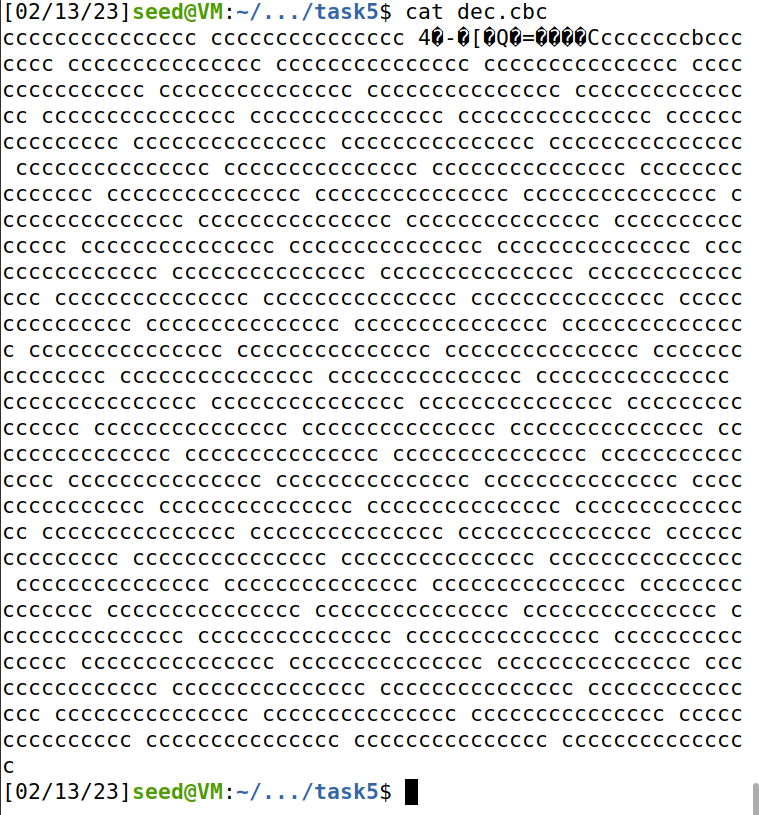
\includegraphics[height=\textheight,width=\textwidth,keepaspectratio]
    {figures/dec_cbc_task5.png}
    \caption{Decrypted text with corrupted bits using CBC mode.}\label{fig:corrupted_cbc}
\end{figure}

\begin{figure}
    \centering
    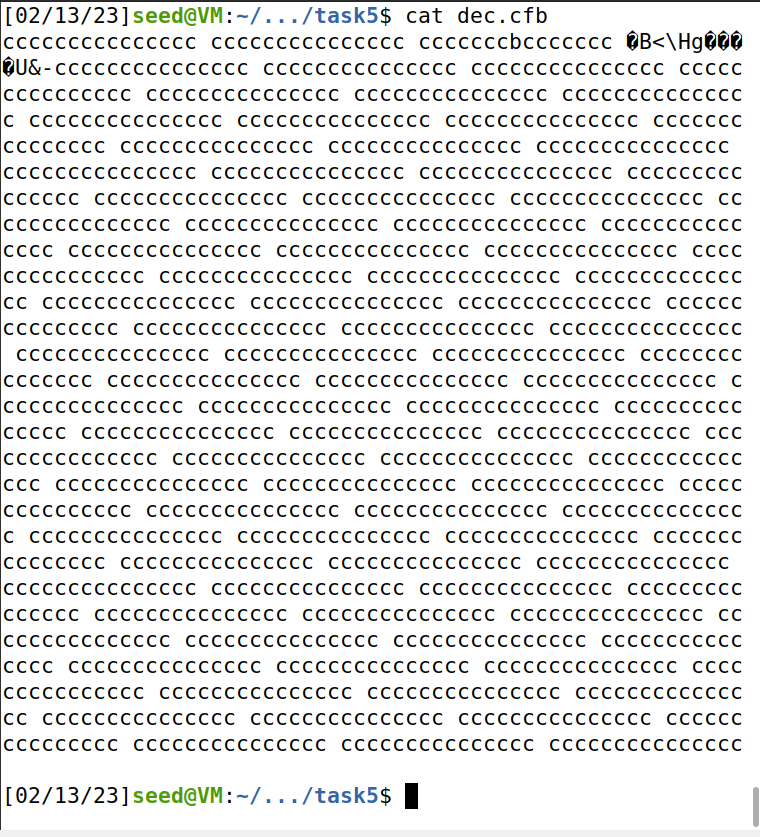
\includegraphics[height=\textheight,width=\textwidth,keepaspectratio]
    {figures/dec_cfb_task5.png}
    \caption{Decrypted text with corrupted bits using CFB mode.}\label{fig:corrupted_cfb}
\end{figure}

\begin{figure}
    \centering
    
\includegraphics[height=\textheight,width=\textwidth,keepaspectratio]
    {figures/dec_ofb_task5.png}
    \caption{Decrypted text with corrupted bits using OFB mode}\label{fig:corrupted_ofb}
\end{figure}

\begin{figure}
    \centering
    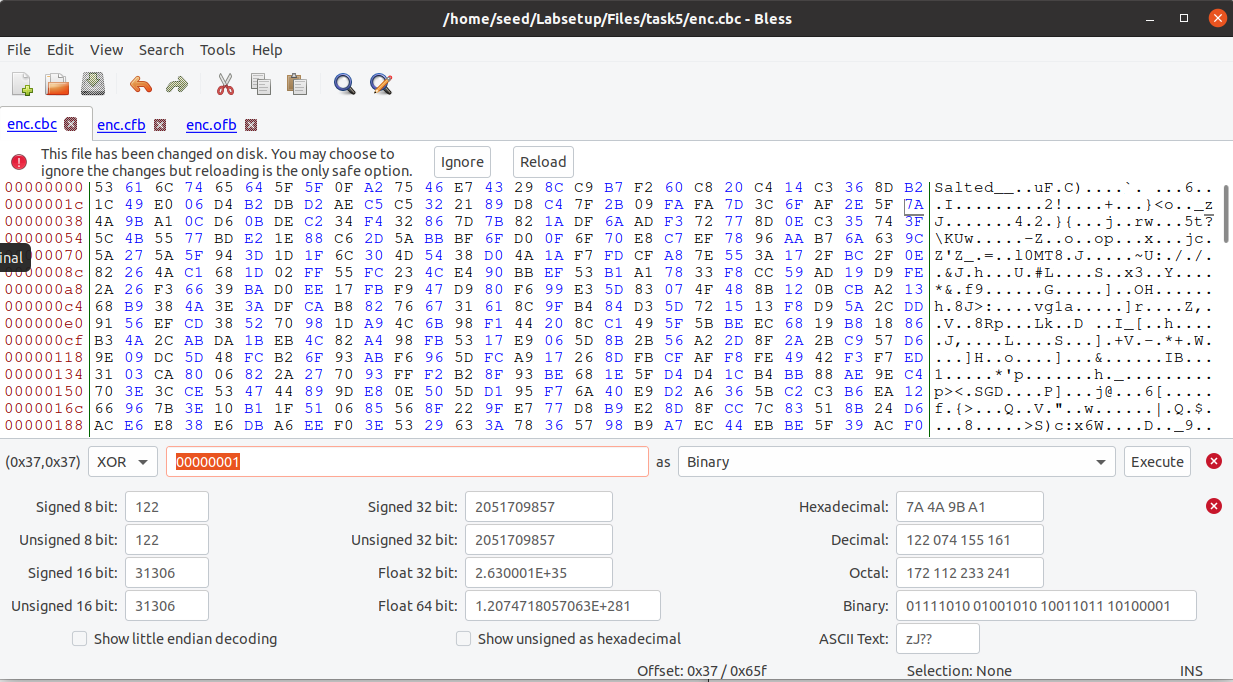
\includegraphics[height=\textheight,width=\textwidth,keepaspectratio]
    {figures/bless_editor.png}
    \caption{Modify the \(55^{th}\) bit using Bless hex editor.}
    \label{fig:bless_editor}
\end{figure}

\begin{figure}
    \centering
    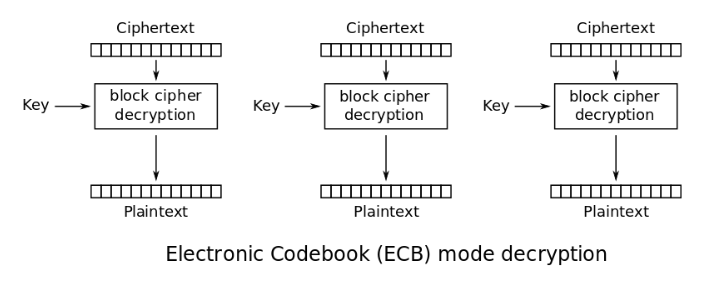
\includegraphics[height=\textheight,width=\textwidth,keepaspectratio]
    {figures/ecb_decryption.png}
    \caption{ECB mode decryption}\label{fig:ecb_dec}
\end{figure}

\begin{figure}
    \centering
    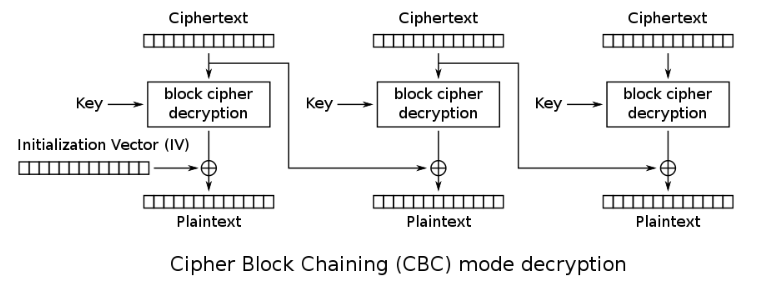
\includegraphics[height=\textheight,width=\textwidth,keepaspectratio]
    {figures/cbc_decryption.png}
    \caption{CBC mode decryption}\label{fig:cbc_dec}
\end{figure}

\begin{figure}
    \centering
    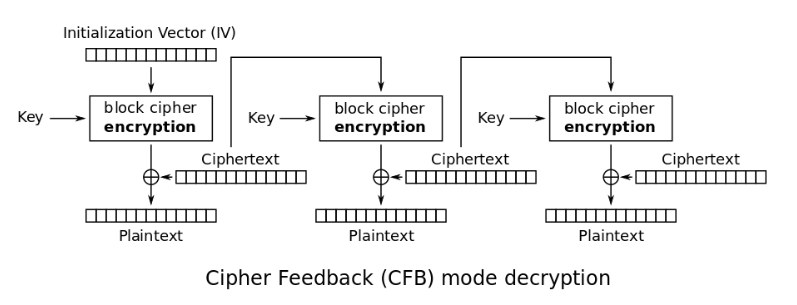
\includegraphics[height=\textheight,width=\textwidth,keepaspectratio]
    {figures/cfb_decryption.png}
    \caption{CFB mode decryption}\label{fig:cfb_dec}
\end{figure}

\begin{figure}
    \centering
    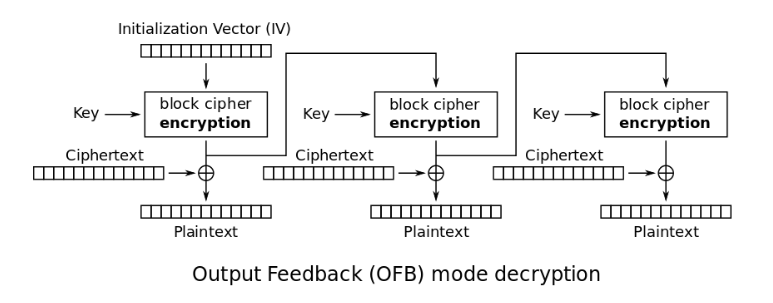
\includegraphics[height=\textheight,width=\textwidth,keepaspectratio]
    {figures/ofb_decryption.png}
    \caption{OFB mode decryption}\label{fig:ofb_dec}
\end{figure}

At first, we created a {\fontfamily{qcr}\selectfont plaintext.txt} that is 1600 bytes long
(see \autoref{lst:plaintext_generation}). The plaintext should be like a chain of strings
``ccccccccccccccc '' (15 `c' characters with a space at the end).
After encrypting it with AES-128 cipher, we used
{\fontfamily{qcr}\selectfont bless} hex editor to modify the \(55^{th}\) byte of the
encrypted file. We did XOR the \(55^{th}\) byte with {\fontfamily{qcr}\selectfont 00000001}
to flip the least significant bit (see \autoref{fig:bless_editor}). Next, we decrypted
files to observe how bit errors behave.

In ECB mode (see \autoref{fig:corrupted_ecb}, \autoref{fig:ecb_dec}), a whole block (16 bytes)
is changed (different
from the original plaintext). Each blocks are decrypted separately as shown in
\autoref{fig:ecb_dec}. Thus, only the block containing the corrupted bit is affected. And
the ciphertext block is fed into the decryptor, so with many substitution, extension, and
permutation steps are performed within the decryptor, the corrupted bits are spread to the
whole block.

In CBC mode (see \autoref{fig:corrupted_cbc}, \autoref{fig:cbc_dec}), the block which holds
the corrupted bit
is changed totally as ciphertext block is fed into the decryptor. However, the next block
is changed at the specific bit according to the position we modified since the current ciphertext
block is only XORed with the output of decryptor of the next block (not being fed into
a decryptor of the next block). In this case, the original character `c' is changed to
`b' as a result of flipping the least significant bit.

In constrast to CBC mode, in CFB mode, the block which holds the corrupted bit changed at a specific
bit according to the position we modified as the corrupted ciphertext block is only XORed
with the output of the decryptor (see \autoref{fig:corrupted_cfb}, \autoref{fig:cfb_dec}).
However, the next block is changed totally as the corrupted ciphertext block is fed into
the decryptor of the next block.

In OFB mode (see \autoref{fig:corrupted_ofb}, \autoref{fig:ofb_dec}), only the current block
is changed at the specific bit according to the position we modified as the corrupted ciphertext
block is only XORed with the output of the decryptor, not being sent to the next block.

After collecting the observations from above tasks and referencing some sources, we created
\autoref{tab:error_effect} to illustrate exactly the effect of bit errors. In that table,
\(C_i\) is the \(i^{th}\) ciphertext block, and \(P_i\) is the \(i^{th}\) plaintext block.

\begin{table}
    \centering
    \begin{tabular}{|l|l|}
        \hline
        Mode & Effect of Bit Errors in \(C_i\)\\
        \hline
        ECB & Random bit errors in \(P_i\)\\
        \hline
        CBC & Random bit errors in \(P_i\)\\
         & Specific bit errors in \(P_{i+1}\)\\
        \hline
        CFB & Specific bit erros in \(P_i\)\\
         & Random bit errors in \(P_{i+1},P_{i+2},\cdot,\) until synchronization is restored.\\
        \hline
        OFB & Specific bit errors in \(P_i\)\\
        \hline
    \end{tabular}
    \caption{The effect of bit errors for block cipher modes~\cite{cipher_mode_wiki,error_prop}.}
    \label{tab:error_effect}
\end{table}

\section{Task 6 --- Launching a Man-In-The-Middle Attack with
a Compromised CA}
%
\begin{lstlisting}[caption=A command generating a Certificate Signing
    Request for the fake Facebook website, label={lst:csr_script_fake_facebook}]
    openssl req -newkey rsa:2048 -sha256 \
    -keyout facebook.key -out facebook.csr \
    -subj "/CN=www.facebook.com/O=Meta Inc./C=US" \
    -passout pass:dees
\end{lstlisting}

\begin{lstlisting}[caption=A command generating a Certificate for the
    fake Facebook website, label={lst:crt_script_fake_facebook}]
    openssl ca -config demoCA_openssl.cnf \
    -policy policy_anything -md sha256 -days 365 \
    -in facebook.csr -out facebook.crt -batch \
    -cert ca.crt -keyfile ca.key
\end{lstlisting}

\begin{lstlisting}[caption={\fontfamily{qcr}\selectfont VirtualHost} entry for
    fake {\fontfamily{qcr}\selectfont www.facebook.com},
    label={lst:virtual_host_entry}]
    <VirtualHost *:443>
        DocumentRoot /var/www/bank32
        ServerName www.facebook.com
        DirectoryIndex index.html
        SSLEngine On
        SSLCertificateFile /volumes/facebook.crt
        SSLCertificateKeyFile /volumes/facebook.key
    </VirtualHost>
\end{lstlisting}

\begin{figure}
    \centering
    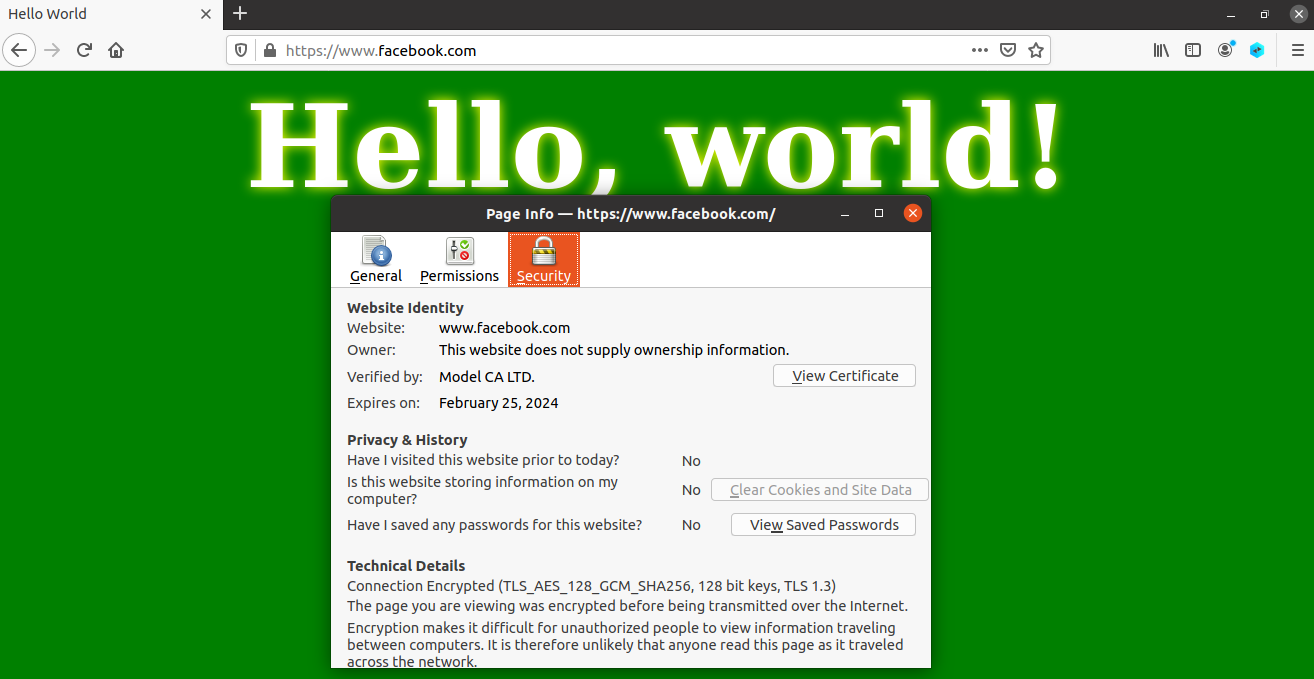
\includegraphics[height=\textheight,width=\textwidth,keepaspectratio]
    {figures/fake_facebook.png}
    \caption{Fake {\fontfamily{qcr}\selectfont www.facebook.com}
    can be accessed without any errors or warnings}
    \label{fig:fake_facebook}
\end{figure}

In this work, we selected the popular
social network Facebook ({\fontfamily{qcr}\selectfont www.facebook.com}) as the
target website. 
As mentioned in the SEED's instruction, the attacker can generate any arbitrary
certificate using the stolen CA's private key. We demonstrate that attack by generating
a certificate that is issued by our root CA for our fake Facebook website. Firstly,
we produced a CSR (see \autoref{lst:csr_script_fake_facebook}). Then we signed using
the compromised CA's private key (see \autoref{lst:crt_script_fake_facebook}). After
we got the certificate stored in {\fontfamily{qcr}\selectfont facebook.crt} and the
private key binding to that certificate {\fontfamily{qcr}\selectfont facebook.key},
we copied those two files into the shared folder {\fontfamily{qcr}\selectfont volumes}.
Next, we added the {\fontfamily{qcr}\selectfont VirtualHost} entry in {\fontfamily{qcr}\selectfont
bank32\_apache\_ssl.conf} (see \autoref{lst:virtual_host_entry}). Consequently, our
fake Facebook website can be visited without any errors or warnings raised by Firefox.
Addtionally, we can see that HTTPS secure connection was shown while we were visiting
the website (see \autoref{fig:fake_facebook}). In conclusion, this experiment shows that
an attacker can do a MITM attack with a compromised root CA.


\appendix

\section{Full list of RSA elements}
\begin{lstlisting}[language=bash, caption=Elements in the RSA algorithm,
    label={lst:rsa_element}]
    publicExponent: 65537 (0x10001) 
    privateExponent: 
        20:7f:43:3a:b5:08:70:ad:9f:60:ef:86:2c:97:c3: 
        fc:c5:2c:29:3c:ce:fc:1a:65:46:88:fa:6d:c0:cd: 
        5b:5a:40:be:77:58:74:4a:3d:62:8b:df:6c:ae:12: 
        8d:13:8f:e5:e3:f0:24:d5:86:e4:52:32:c7:1a:49: 
        09:11:d9:74:8c:da:37:e1:08:5b:d8:f7:76:64:58: 
        90:d2:4a:f9:9e:16:b8:1c:b6:db:d0:d3:eb:18:9a: 
        b0:fe:f5:09:b7:11:1f:01:fc:7b:2d:87:a2:b4:58: 
        c4:d6:65:a3:c0:88:1f:7d:7c:22:ac:33:d3:95:38: 
        bd:ef:7d:44:bb:fa:93:65:d4:2a:c1:4e:56:6c:8d: 
        be:8f:bc:21:af:af:30:c7:73:b5:92:ff:0d:88:b8: 
        bb:d6:b0:d2:43:84:06:47:c1:bd:17:4c:57:50:1b: 
        26:c4:c3:a4:f2:1b:86:e1:26:6a:06:63:f2:81:dd: 
        98:81:0d:f3:2e:8b:c5:44:ef:46:67:8e:51:33:b6: 
        0a:43:aa:42:a7:4b:1c:51:46:2e:7d:ae:31:aa:f6: 
        c3:82:c5:92:26:e5:9e:00:c4:0e:59:00:b7:ae:28: 
        8c:40:80:44:b6:06:01:4e:25:b1:92:dc:31:6d:12: 
        f5:90:70:70:10:f0:97:e3:8a:e1:bc:11:a5:1c:ce: 
        0e:18:e7:84:a4:10:8c:6c:17:d3:8d:d0:47:71:b3: 
        e0:f9:bd:72:af:e4:88:4f:74:af:ac:f5:5d:9b:d0: 
        8d:ab:97:89:03:93:76:79:a9:7b:09:7d:0f:e1:3f: 
        80:62:1e:ae:dd:05:63:5d:1c:05:97:e8:e3:11:dd: 
        3a:96:98:61:8c:83:6a:3f:f7:20:7a:d1:2a:05:da: 
        d6:ef:1d:7a:cd:a4:fc:6b:9f:93:a9:2f:9b:be:48: 
        b8:31:bc:44:0b:8d:dd:a3:1d:dd:13:a2:9c:b8:d9: 
        c2:6d:23:5a:98:36:e5:0d:2b:43:e9:a8:32:52:c3: 
        b5:e4:88:70:b7:0c:68:db:f2:2d:6c:70:8b:63:59: 
        77:71:80:fb:ff:18:fc:a5:61:ba:6e:d1:59:e7:95: 
        9b:4b:1e:d9:01:52:e7:dd:3f:ba:3e:b2:8f:81:16: 
        c0:9a:2d:5c:67:33:93:fd:d2:ee:39:36:0c:92:24: 
        f4:7f:2e:73:cb:14:da:b2:cf:78:38:6a:0b:8f:dd: 
        42:03:59:35:7b:c6:04:50:36:4e:e4:1e:39:f0:4c: 
        be:f8:72:2d:93:2d:c2:ac:ff:ce:95:ca:37:10:de: 
        4d:19:81:a6:3e:ce:52:48:a2:9d:9d:b1:e9:e4:56: 
        0f:36:79:e0:ef:cf:ad:d5:cc:73:c0:78:bf:be:b3: 
        04:01 
    prime1: 
        00:f8:7e:56:50:cf:97:5d:ec:0a:08:e0:94:9a:f9: 
        7e:fb:13:23:e4:29:9b:a7:9f:3c:4e:70:ca:a9:7d: 
        87:51:52:2d:f9:3f:23:ff:95:66:b6:d7:46:c9:e8: 
        79:dc:41:08:96:03:96:77:31:28:4b:12:3c:b2:b9: 
        25:cd:fa:54:49:e7:be:62:b8:fe:00:14:40:91:b6: 
        9f:78:77:5a:40:0d:cb:37:ff:94:27:1c:07:e0:46: 
        9c:cd:79:13:f0:54:8c:f1:9d:a7:3f:41:e7:b0:97: 
        70:e8:bb:a3:ac:7c:75:dc:ed:d6:33:a4:c4:63:0c: 
        cb:15:9a:f5:c2:44:21:8c:a2:e7:90:9b:1b:09:c8: 
        23:ef:2a:3f:5e:ed:af:e9:03:a0:6b:c6:5f:3c:b6: 
        a3:14:9a:45:cc:6e:b1:f7:a5:c8:79:99:74:48:f1: 
        3a:a2:81:75:58:04:32:82:42:36:59:22:2a:43:bb: 
        1b:51:e1:3b:c1:50:91:83:ff:7f:1c:ce:24:06:b1: 
        12:87:fd:d3:f4:4a:1b:9a:fe:6f:86:23:39:2f:5a: 
        34:33:e9:40:32:b0:4f:ae:20:62:65:68:64:87:d4: 
        8f:de:f6:0d:68:e8:c0:c7:81:a1:f1:91:8a:43:b7: 
        9a:e1:97:01:3b:7b:65:fc:3b:25:a9:8f:35:16:6d: 
        2d:a1 
    prime2: 
        00:d5:1a:26:04:9c:d5:4f:64:53:8d:cd:82:30:5b: 
        71:fb:a2:18:41:b9:20:2f:fd:03:2a:82:da:c2:7d: 
        c2:56:93:82:b3:9b:a5:b8:e3:05:6c:3a:6a:ec:1c: 
        49:5f:73:71:25:10:c2:56:25:14:31:37:c2:26:e1: 
        75:22:5c:1c:15:f7:5a:43:21:27:5f:0a:5c:41:05: 
        8d:86:70:6a:7d:bb:80:8c:2e:bc:d5:4f:5b:56:38: 
        ac:35:88:3d:ec:7e:28:f1:2c:a9:01:4b:4e:fd:2e: 
        94:bb:1c:4c:b5:c3:02:c0:25:5d:1b:68:1b:36:6c: 
        bb:76:36:d8:59:82:9b:fb:f9:b7:94:7d:4a:c7:b0: 
        b7:e8:f3:32:bc:28:44:74:07:16:86:2a:ca:1c:8c: 
        d2:96:c9:1e:f5:39:a2:14:62:36:3e:7c:07:eb:c9: 
        6a:5f:ba:fc:3a:1f:7f:68:a9:01:92:df:d7:8b:ad: 
        bb:a0:e9:99:78:63:62:73:66:84:2d:3c:80:e6:9d: 
        20:7a:59:4b:8a:2f:ae:78:7d:b1:3d:74:31:15:92: 
        ee:47:38:97:7c:c5:98:31:b0:ba:cf:68:e2:52:ab: 
        88:b4:84:09:db:e9:33:a4:12:ea:ef:74:76:79:fb: 
        4e:5f:c1:80:4b:84:67:45:fe:4d:a0:a0:cd:d6:74: 
        bc:cd 
    modulus: 
        00:ce:da:7f:8d:3b:f3:69:60:13:75:21:ca:fe:28: 
        97:af:12:52:b5:3b:ad:df:36:bc:31:af:43:ff:15: 
        f5:29:c3:09:2a:f7:9e:6c:ac:4c:b3:40:4c:32:76: 
        22:7d:77:78:93:b0:2f:f5:00:7d:8f:3e:6f:9f:41: 
        72:0f:63:51:e9:7b:18:95:76:c1:a9:b4:7e:e3:d9: 
        62:97:0b:a1:9d:2a:c6:45:4e:8b:73:5c:7c:d0:c5: 
        76:fd:41:97:96:7a:cc:a1:fd:e6:12:26:a8:ae:f1: 
        5d:ea:7f:2a:9e:e2:a8:47:bf:71:95:31:4a:fc:0c: 
        3d:bd:c4:9a:db:d4:38:df:96:5d:e6:ac:e1:c2:35: 
        cf:58:0e:30:91:e5:c3:f0:a6:66:f6:6b:87:13:17: 
        07:de:f7:5d:1d:59:11:f2:5e:7b:d8:0b:5f:a4:69: 
        7c:17:de:0b:c7:41:0e:58:a1:d8:e4:ab:69:72:1f: 
        08:69:c9:a8:95:7e:ae:57:89:f5:8a:69:f0:4e:06: 
        25:be:33:d4:65:7b:dd:e0:7b:63:40:58:3c:0e:26: 
        cc:71:9d:f6:93:1b:71:b3:60:eb:e3:48:94:67:cd: 
        e1:3a:81:9a:af:32:fd:32:d3:6b:34:ec:a6:65:ac: 
        f6:b7:7b:46:a0:5b:84:19:2a:6f:eb:7c:67:76:b6: 
        48:48:c9:f4:b8:4b:9b:61:41:69:05:9c:58:4a:29: 
        b2:e4:f8:42:92:9b:d2:3a:a6:01:ab:eb:a6:88:36: 
        07:db:29:ea:94:1b:f5:7e:42:e9:85:79:00:6c:3f: 
        a6:84:d0:aa:c0:d5:a3:f8:97:37:ab:c6:72:0d:0a: 
        8b:33:66:90:b9:4c:4d:76:38:7c:12:53:06:dd:0c: 
        24:86:5b:1c:87:28:00:0c:54:18:05:38:2c:a7:63: 
        2a:1c:ea:0d:98:de:a9:2a:de:e6:2a:7f:00:97:6f: 
        ac:d7:77:08:77:88:ac:ce:0c:46:59:06:8c:ac:8d: 
        7d:b8:14:d4:1f:a6:58:bd:57:f4:2d:55:2e:79:02: 
        b9:60:31:d5:c6:72:55:4d:3c:94:28:89:9b:72:c5: 
        42:bc:4d:28:38:67:3f:ed:cf:5a:55:01:ff:f5:3c: 
        3e:90:be:28:51:75:e4:b8:1e:69:08:16:48:90:d5: 
        37:46:d7:04:97:66:df:42:ba:2f:fb:ed:34:b6:ad: 
        79:9b:d9:d7:a4:17:ec:90:58:f8:6d:01:fa:6c:d1: 
        86:47:68:a9:73:91:1c:24:9c:72:85:60:66:2f:0f: 
        8b:62:2b:37:40:0e:a1:72:81:2f:42:b1:45:d7:eb: 
        a5:79:2e:79:e8:9b:1a:cb:9a:cc:16:52:41:85:65: 
        e3:c5:ed     
\end{lstlisting}

\printbibliography{}

\end{document}